\documentclass[twocolumn, 11pt]{extarticle}
\usepackage{amsmath}
\usepackage{lineno,hyperref}
\usepackage[table,x11names,dvipsnames,table]{xcolor}
\usepackage{authblk}
\usepackage{subcaption,booktabs}
\usepackage{graphicx}
\usepackage{multirow}
\usepackage[nolist,nohyperlinks]{acronym}
\usepackage[superscript]{cite}
\usepackage{tabularx}
\usepackage{float}
\usepackage[group-separator={,}]{siunitx}
\usepackage{geometry}
 \geometry{
 a4paper,
 papersize={210mm,279mm},
 left=12.73mm,
 top=20.3mm,
 marginpar=3.53mm,
 textheight=238.4mm,
 right=12.73mm,
 }


\setlength{\columnsep}{6.54mm}

%\linenumbers %%% Turn on line numbers here

\renewcommand{\familydefault}{\sfdefault}

\captionsetup[figure]{labelfont=bf,textfont=normalfont}


%%%% comment out the below for the other title option
\makeatletter
\def\@maketitle{
\raggedright
\newpage
  \noindent
  \vspace{0cm}
  \let \footnote \thanks
    {\hskip -0.4em \huge \textbf{{\@title}} \par}
    \vskip 1.5em
    {\large
      \lineskip .5em
      \begin{tabular}[t]{l}
      \raggedright
        \@author
      \end{tabular}\par}
    \vskip 1em
  \par
  \vskip 1.5em
  }
\makeatother




\begin{document}


\title{State of relation extraction using LLMs: A report }

\author{Vangmay Sachan\thanks{vangmay.sachan16@email.com}}
\author{Yanfei Dong \thanks{}}

\affil[1]{National University of Singapore}
\affil[2]{Odyssey 2023/2024}

\setcounter{Maxaffil}{0}
\renewcommand\Affilfont{\itshape\small}

\date{}  
\maketitle


\begin{abstract}
Relation Extraction is one of the three key tasks within the field of information extraction. Relation extraction aims to extract contextual relation between entities from plain natural language texts. Large language models have demonstrated impressive ability to understand the task and generate remarkable results. Because of their ability, numerous works have proposed different techniques and methods to train LLMs in the task of relation extraction. 

In this report, we survey some of the advancements in this field. First, we present an overview of techniques and benchmarks used for relation extraction then we categorise them and analyse the most promising methods. We also recognize the fallbacks and possible future directions for the field. 

 
\end{abstract}

\section{Introduction}

Information extraction is a crucial domain in natural language processing which converts unstructured data into structured knowledge (eg, entities, relations and event) and serves as a foundational requirement for other downstream tasks. It comprises three key tasks: Named Entity Recognition (NER), Relation Extraction (RE), Event Extraction (EE). In this paper, we are going to focus on the sub-domain of Relation Extraction. The surge of large language models (LLMs) (eg, GPT-4 and Flan T5) has promoted the development of NLP, due to their extraordinary capabilities in text understanding and generation. Because of such advancements, there has been a wave of interest in generative methods to solve relation extraction. Because of their wide language ability, LLMs are able to understand and account for the complexity of human language which makes them more practical in real world applications as compared to other methods. They are also easily able to handle schemas as varying lengths of input without degradation in performance unlike their predecessors (RNNs)

In this report, we provide an exploration of the usage of LLMs in generative RE. We categorise LLM techniques into 3 taxonomies: One-Shot / Few-Shot, Alignment, UIE. 


\section{Preliminaries of relation extraction }

\subsection{What is relation extraction}

Relation extraction is the task of extracting contextual information from unstructured data. Such as if a text says “John works for apple” then the output should be(“John”, “works\_for”, “apple”).

\textbf{Relation Classification}

Refers to classifying the relation type between two given entities

\textbf{Relation Triplet}

Refers to identifying the relation type and the corresponding head and tail entity spans

\textbf{Relation Strict}

Refers to giving the correction relation type, the span and the type of head and tail entity

 

\subsection{Document Level + Sentence Level}

Relation extraction is being studied upon at two different levels, document level and sentence level. Document level is more challenging because the model needs to look at “evidence” which can be present throughout the entire document no matter how long it is.  

\subsection{Overview of current benchmarks}


There are several benchmarks being used to evaluate relation extraction. Most representative of them are


\begin{table}
    \centering
    \begin{tabular}{|c|c|c|} \hline 
         Dataset&  SoTA Model& Score\\ \hline 
         DocRED&  DREEAM& 67.530\\ \hline 
         TACRED&  RAG4RE& 86.600\\ \hline 
         NYT&  UniRel& 93.700\\ \hline 
         CoNLL04&  REBEL& 76.650\\ \hline 
 ACE 2005& PL Marker&73.000\\ \hline
    \end{tabular}
    \caption{Caption}
    \label{Some benchmarks along with their current representative model}
\end{table}

\textbf{DocRED}

Document-Level Relation Extraction Dataset is a relation extraction dataset constructed from Wikipedia and Wikidata. Each document in the dataset is human-annotated with named entity mentions, coreference information, intra- and inter-sentence relations, and supporting evidence. DocRED requires reading multiple sentences in a document to extract entities and infer their relations by synthesising all information of the document. Along with the human-annotated data, the dataset provides large-scale distantly supervised data.

\textbf{TACRED} 
is a large-scale relation extraction dataset with 106,264 examples built over newswire and web text from the corpus used in the yearly TAC Knowledge Base Population (TAC KBP) challenges. Examples in TACRED cover 41 relation types as used in the TAC KBP challenges (e.g., per:schools\_attended and org:members) or are labelled as no\_relation if no defined relation is held. These examples are created by combining available human annotations from the TAC KBP challenges and crowdsourcing.

\textbf{New York Times Annotated Corpus} contains over 1.8 million articles written and published by the New York Times between January 1, 1987 and June 19, 2007 with article metadata provided by the New York Times Newsroom, the New York Times Indexing Service and the online production staff at nytimes.com. The corpus includes:

\begin{itemize}
    \item Over 1.8 million articles (excluding wire services articles that appeared during the covered period).
    \item Over 650,000 article summaries written by library scientists.
    \item Over 1,500,000 articles manually tagged by library scientists with tags drawn from a normalised indexing vocabulary of people, organisations, locations and topic descriptors.
    \item Over 275,000 algorithmically-tagged articles that have been hand verified by the online production staff at nytimes.com. As part of the New York Times' indexing procedures, most articles are manually summarised and tagged by a staff of library scientists. This collection contains over 650,000 article-summary pairs which may prove to be useful in the development and evaluation of algorithms for automated document summarization. Also, over 1.5 million documents have at least one tag. Articles are tagged for persons, places, organisations, titles and topics using a controlled vocabulary that is applied consistently across articles. For instance if one article mentions "Bill Clinton" and another refers to "President William Jefferson Clinton", both articles will be tagged with "CLINTON, BILL".
\end{itemize}
\textbf{CoNLL04} dataset is a benchmark dataset used for relation extraction tasks. It contains 1,437 sentences, each of which has at least one relation. The sentences are annotated with information about entities and their corresponding relation types.

[Table of representative models to benchmarks]

\subsection{Overview of current approaches}


\subsubsection{Few shot / One-shot}
Few Shot approaches can be categorised as a prompt engineering approaches. The main aim is to craft elaborate prompts and also give the model examples and expect the model to follow those examples when producing the output. Some studies have experimented with Chain of thought style examples which use logical thinking in the same manner as humans do and have gained good results from it. Besides that, some approaches also involve fine-tuning the model on those prompts for complex situations which require more elaborate instructions. 

\subsubsection{Alignment}

There is a key issue in Relation extraction, which is that it is rare to find datasets whose design is suitable for relation extraction. Many researchers have hypothesised that because of this performance of LLMs in relation extraction is not as good as their performance in other tasks. This is especially observed in zero shot scenarios. To combat this issue, the approach being taken is to formulate relation extract as other IE tasks which are prevalent in a higher number of datasets. 

\subsubsection{Universal Information Extraction}
As mentioned for Alignment tasks, that very few datasets are built keeping relation extraction in mind, this is not only true for RE but also several other tasks. The problem with the field of information extraction is that despite the fact that these tasks are very “close” in the sense they require the same abilities but the scientific community has came up with different infrastructures like datasets, models, techniques and these tasks have become very disconnected from each other. Universal information extraction or UIE for short is a framework that was first explored in the paper (Lu et al., 2022). Which aims to unify these tasks to ensure we are able to share knowledge from one task to another. Basically, build a framework that can do all tasks within the domain of Information extraction.

\section{Techniques of LLMs for Generative RE}
In this section we categorise recent methods based on their technique, including Prompt design, Zero Shot learning, Data augmentation, supervised fine tuning and UIE. We also give an analysis of the recent methods by looking at papers and where does their future direction lead to.

\subsection{Prompt Design}
Prompt engineering is a technique employed where instead of altering model parameters, we try to design creative prompts to exploit LLMs detailed understanding of natural language to guide the behaviour of our model. The craft of prompt design has proven successful in a variety of areas, similarly it plays an effective role in relation extraction. 


\subsubsection{Chain of thought (CoT)} 
CoT (Wei et al. 2022b) is a strategy used for LLMs to enhance their performance. It involves adding detailed explanations in the form of a step-by-step reasoning chain which is similar to the human thought process. Ongoing research has explored further into the effectiveness of Chain of thought for Relation Extraction tasks. (Wadhwa et al., 2023) Proposed a distillation technique in which they target RE labels with CoT style explanations elicited from GPT-3 used to fine-tune FLAN-T5 large. A 2-step approach was introduced, leveraging GPT-3 prompts were generated that used chain-of-thought style explanations along with target labels and later the prompts were used to fine-tune Flan-T5 large and as a result, it had a 5 - 10 increase in micro F1 score as compared to SoTA Rebel model (Huguet Cabot and Navigli, 2021).

The paper highlighted that although Flan-T5 is not as capable in a few shot setting but supervising and fine-tuning it using chain of thought style explanations generated using Chat-GPT yields SoTA results even outperforming GPT-3 which is a much larger model as compared to Flan-T5 large. Moreover, A notable issue was addressed regarding evaluating generated approaches to tasks such as RE using manual human evaluation.

The authors proposed using a few short CoT style prompts, but that led to a performance below SoTA. So the authors proposed fine-tuning Flan T5 largely on a chain of thought style explanations generated by GPT-3 and this led to a major increase across the representative datasets.

\begin{itemize}
    \item ADE: 9.97 point gain in micro F1 score over the existing fully supervised generative SOTA REBEL.
\end{itemize}
\begin{itemize}
    \item CoNLL: 5.42 point gain
    \item NYT : 3.37 point gain
    \item Fine tuning Flan T5 with both train labels and CoT explanations produced by GPT-3 yields SOTA performance across RE dataset by 5 - 10 micro F1
\end{itemize}

\begin{figure}
    \centering
    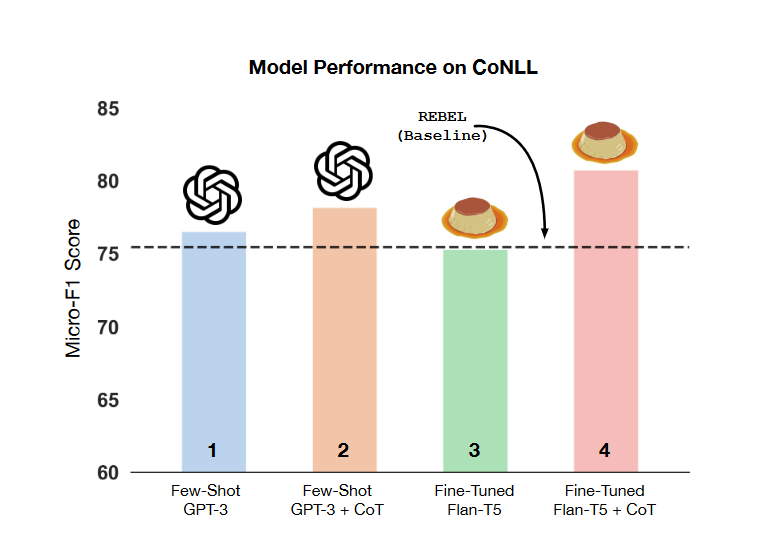
\includegraphics[width=1\linewidth]{RE_.png}
    \caption{(Wadhwa et al., 2023) Figure 1 }
    \label{Zero Shot results}
\end{figure}

\textbf{Challenges}
Challenges were faced in automating the evaluation of the model due to the complexity of language. Example if the model is prompted to list all drugs and adverse events it may yield "Aspirin: Stomach ache, chest pain". While another model may return "Side effects of aspirin may include stomach pain and pain in the chest". This challenge was overcome by enlisting human annotators to judge whether the model output conveys the same information as the reference target then compared them to the automated evaluation and categorised the prediction into false-positives, false-negative to compute F1 scores. 

\subsubsection{Document Level RE}
(Li et al., 2023) introduces a sophisticated approach to document level relation extraction (DocRE) through automated annotation leveraging advanced techniques like NLI modules to enhance LLMs. By integrating GPT-3.5 and GPT-4 the framework generates relation triples from text prompts, initially with constraints on entity and relation types that were later relaxed to enhance flexibility and accuracy. These triples are then aligned with predefined annotations in the ReDocRED dataset. Experimental results demonstrate the framework’s effectiveness while LLM-generated triples exhibit variability from ground truth, incorporating NLI significance improves alignment, achieving notable recall rates like 5.77 in matching Re-DocRED triples. The resulting dataset, DocGNRE, is enriched with these augmented triples, enhancing the completeness of DocRE datasets. This augmentation is shown to improve the performance of SoTA DocRE datasets in subsequent experiments, underscoring the framework’s potential despite challenges like noise in LLM-generated data and the need for robots quality assessment methodologies. 

\subsubsection{Future directions}
Although distillation using Chain of thought style explanations yielded impressive results (Wadhwa et al., 2023), the paper still has some areas where it could be improved. GPT-3 style explanations were not evaluated for correctness More complex RE datasets were excluded, evaluating them on this approach could have led to more insights. The authors did not consider N-ary relations and did not fine-tune GPT3. One interesting observation in the paper was that a small LLMs was able to outperform GPT3 using clever technique, one research direction can be the investigation of other previous tasks looking to find if such observation is true for other smaller LLMs. (Li et al., 2023) Also faced limitations with the number of generated triples being upper bounded.

\subsection{Alignment}
Fine tuning LLMs on large scale datasets substantially improves their performance on a wide range of NLP tasks, especially in a zero shot setting. Researchers found that this is not the case for all tasks, especially RE (Zhang et al., 2023).  Advanced instruction-tuned LLMs fail to outperform small LMs on relation extraction. Researchers have hypothesised that this occurs because of RE’s low incidence in instruction-tuning datasets, making up less than 1\%. This has led to methods that formulate RE as other tasks in NLP such that they can benefit from the presence of these tasks in current datasets. 

\begin{figure}
    \centering
    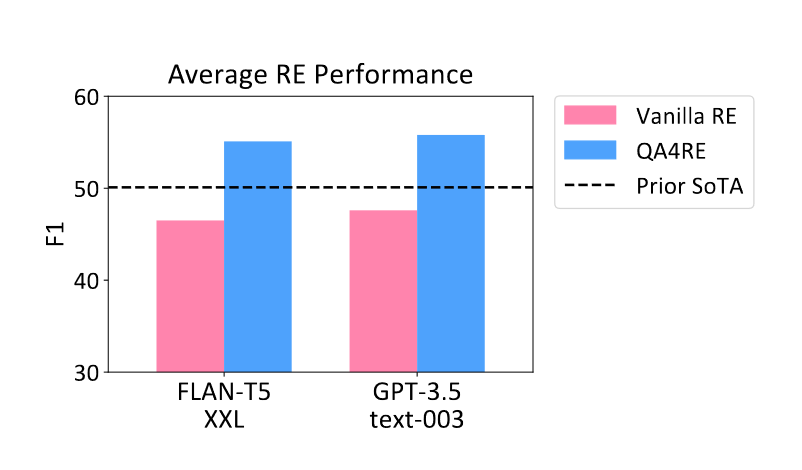
\includegraphics[width=1\linewidth]{RAG4RE_results.png}
    \caption{(Zhang et al., 2023) Figure 1 shows the finding that strong Strong instruction-tuned
LLMs underperform prior zero-shot RE methods us-
ing the standard (vanilla) RE formulation. Meanwhile, QA4RE enables these models to perform better than prior State-of-the-art }
    \label{RAG4RE Results}
\end{figure}
\subsubsection{QA4RE}
(Zhang et al., 2023) examines the capability of LLMs in identifying the relationship between entities in a sentence. The paper introduces a QA4RE framework to address the low incidence issue which aligns RE with multiple choice question answering (QA), this is because the task appears much more frequently in most instruction tuning datasets. 
QA4RE brings significant gains over standard RE formulation on validating its effectiveness and the hypothesis regarding low incidence of RE. The framework enabled Davinci003 and FLAN-T5-XXLarge to achieve an average of 8.2\% and 8.6\% absolute improvement in F1 score. 

The paper investigates instruction tuned LLMs on four real world RE datasets and their limited performance on RE might be due to low incidence of RE tasks in instruction tuning datasets. They reformulate RE as multiple choice QA in efforts to exploit its high prevalence in instruction tuning datasets and demonstrate its robustness to diverse prompt designs, they also show how the framework is transferable and consistent across models of different sizes from 80M to 175B. 

The experiments required the model to identify the relation between a head entity ($E_h$) and tail entity ($E_t$) expressed in $S$ from a set of predefined relation types. 

They integrate the head and tail RE entities into relation templates and use them as multiple choice options. The sentence is used as context to the QA system and to ensure fair comparison with previous work, they apply type restrictions to eliminate options for relation types that are not compatible with the entity types of head and tail entities. 

For baseline, they used  NLI (Sainz et al., 2021) which reformulates RE as a natural language inference task and leverages several LMs fine tuned on MNLI dataset and
SuRE (Lu et al., 2022) frames RE as a summarization task and utilises generative LMs such as BART-Large (Lewis et al., 2020) and PEGASUS Large (Zhang et al., 2020), achieving competitive results in few-shot and fully-supervised settings.

By reformulating RE as QA, the framework improves upon the vanilla RE formulation on all the LLMs and most datasets, making them much stronger zero-shot relation extractors.In particular, text-davinci-003 and FLAN-T5 XL and XXL are able to outperform the prior SoTA, NLI DeBERTa, by a large margin. QA4REbrings the largest gain on the best LLM in each series (text-davinci-003 and FLAN-T5 XXL), showing that stronger LLMs may benefit more from our framework. Consistent and substantial improvements can also be observed in other FLAN-T5 models and the full test set. These findings strongly support the hypothesis that aligning underrepresented tasks such as RE unlocks LLMs’ ability to solve low frequency tasks.

\subsubsection{RAG4RE}
A key issue identified by researchers exploring the use of LLMs for RE was the occurrence of hallucinations. LLMs are said to hallucinate when they perceive patterns or objects that are non-existent, leading to nonsensical or inaccurate outputs. (Efeoglu \& Paschke, 2024) propose Retrieved-Augmented Generation-based Relation Extraction which aligns RE as a Information retrieval task. The model leverages prominent LLMs including FLANT5, Llama2 and mistral and is evaluated on established benchmarks like TACRED, TACREV, Re-TACRED and semEval RE datasets.  

The findings conclude RAG based RE approach has the potential to outperform both simple query known as vanilla LLM prompting and existing best performing RE approach from previous studies and while decoder only LLMs still encounter hallucination issues on these datasets the RAG based RE approach effectively mitigates the problem, especially when compared to the results obtained from the simple query. 

\begin{figure}
    \centering
    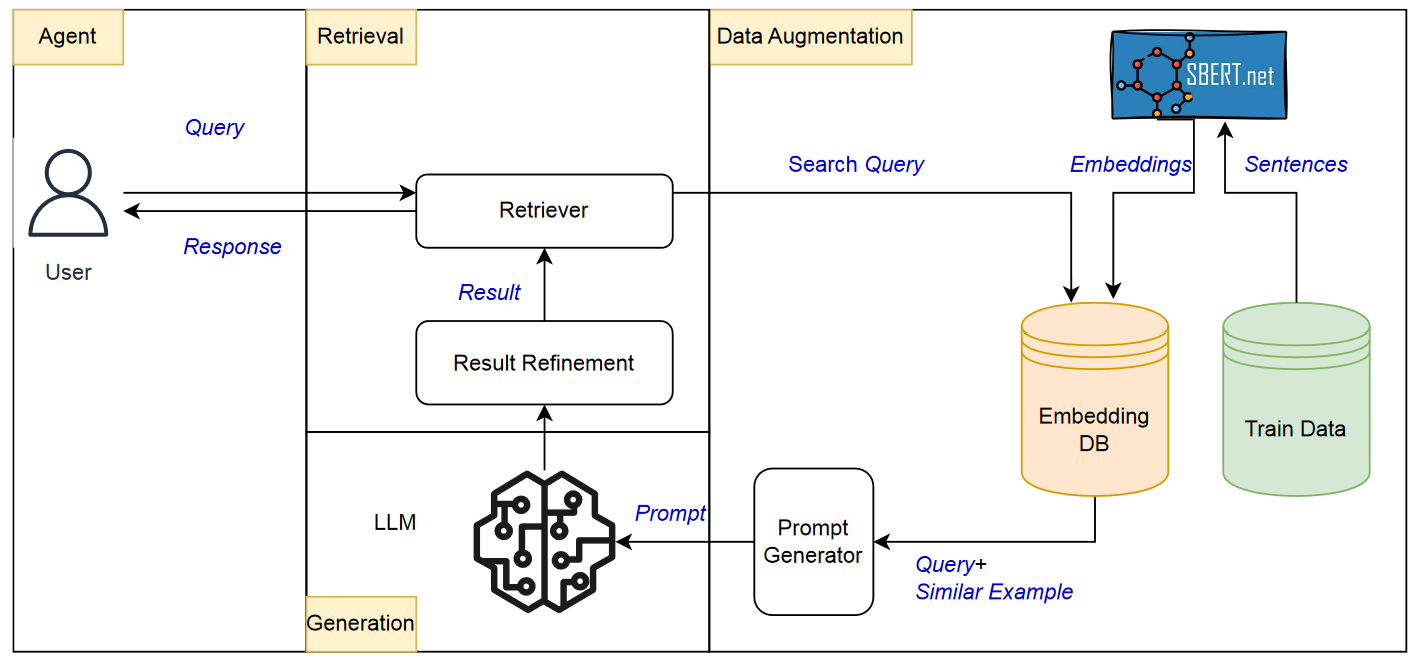
\includegraphics[width=1\linewidth]{RAG4RE_pipeline.png}
    \caption{Efeoglu and Paschke (2024) Figure 2, overview of RAG Based relation extraction pipeline }
    \label{RAG4RE Framework}
\end{figure}

The system operates by receiving a user query and a pair of entities that may be related. This query is then passed to a data augmentation module, which utilises a sentence BERT (SBERT) model to compute embeddings for both the query and a large database of training sentences. Using cosine similarity, the module identifies semantically similar sentences from the database and extends the original query with these relevant sentences. These augmented queries, enriched with additional context from the training data, are then passed to a prompt generator. The prompt generator combines the original query with the retrieved sentences to generate a more comprehensive response for the user. This process effectively enhances the user query by leveraging embeddings and similarity scores to incorporate relevant information from a vast dataset, enhancing the relevance and depth of the system's responses. Enhancing the query allows the model to gain more information and reduce the risk of hallucinations occurring, providing robustness to the otherwise unpredictable nature of LLMs. 

\textbf{Results} \\
RAG4RE approach has improved F1 scores on benchmark datasets whose predefined relations are coming from a given sentence tokens (TACREDm TACREVm Re-TACRED) when comparing its results to those of a simple query. RAG4RE has achieved remarkable results when comparing its performance to that of the simple query. The highest F1 scores amongst the results at Table 2 have been accomplished 86.6\%, 88.3\% and 73.3\% of F1 scores on the TA-CRED, TARCEVA and Re-TACRED, respectively. These outstanding scores were achieved through the integration of the Flan T5-XL model into the Generation module.

\begin{figure}
    \centering
    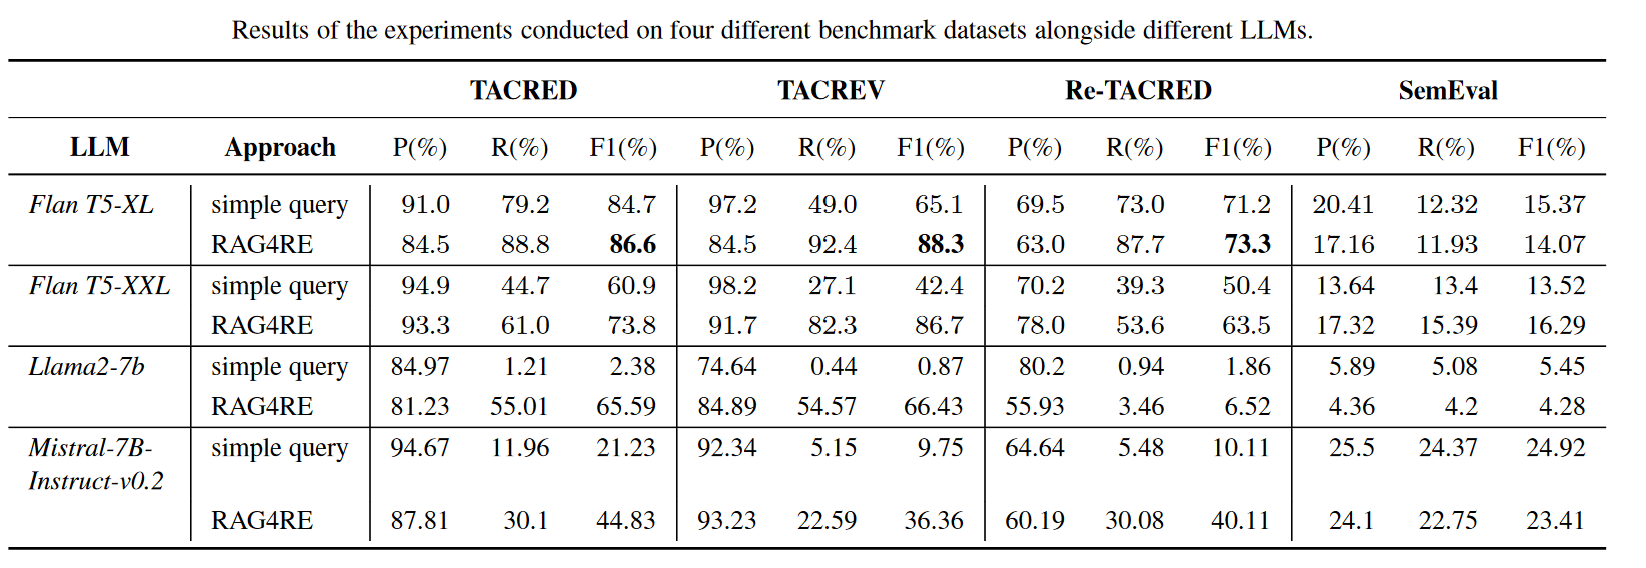
\includegraphics[width=1\linewidth]{RAG_results.png}
    \caption{Efeoglu and Paschke (2024) Results of the experiments conducted on four different benchmark datasets alongside different LLMs }
    \label{RAG results}
\end{figure}
\begin{figure}
    \centering
    \includegraphics[width=1\linewidth]{RAG_results_2.png}
    \caption{ Efeoglu and Paschke (2024) Figure 5 }
    \label{RAG Results}
\end{figure}


\subsubsection{Future directions}
Looking at the successful results, future work might involve looking at other under representative tasks and try to align them to pre-existing tasks. We should definitely try experiment by using QA4RE framework using other LLMs such as the OPT series. (Efeoglu \& Paschke, 2024) plans to extend their approach (RAG4RE) to real world dynamic learning scenarios and evaluate it using real world datasets. 


\subsection{Universal Information Extraction}
The problem with having different models and different datasets for information extraction tasks is that it reduces knowledge sharing between tasks which are essentially similar and could accelerate progress since one task could benefit from techniques learned for other tasks in information extraction. Universal Information Extraction or UIE is a framework proposed that aims to unify information extraction.

\subsubsection{Unified Structure general for information extraction}
(Lu et al., 2022) Agrees with the notion that IE techniques are specialised which leads to dedicated infrastructure (models, datasets, benchmarks) for each task which hinders the rapid architecture development and knowledge sharing. 
By recognizing that all IE tasks can be viewed as structure transformations with 2 atomic operations spotting and associating, they develop Structured extraction language (SEL) to model the structure and adaptively generate targeted structures using Structural schema instructor (SSI)
 \begin{itemize}
     \item \textbf{Spotting} - Involves locating spans given a semantic type. eg. location in a sentence. “I went to France”, ans = France
     \item \textbf{Associating} - Connects spans by assigning them with semantic roles in pre defined schemas. “Steve Jobs” “Apple” = “Work\_for”. The model is then pretrained using several benchmarks to learn key IE tasks.
 \end{itemize}

SEL proved to be advantageous because it uniformly encodes varying IE structures, hence different IE tasks can be modelled as the same text to structure generation process. 
Furthermore, SSI constructs a schema based prompt and is used as a prefix during generation, it contains 3 types of tokens (SpotName, AssoName and Special symbols) which then indicate the model of what kind of task it is supposed to accomplish. 
The model is then pre-trained on several tasks, the datasets are pre-processed such that given a prompt output from SSI, the output expected from the model is in SEL. 

\textbf{Results}
UIE provides an effective universal architecture for IE, the model achieves SoTA performance on nearly all datasets and tasks, even without pre-training (SEL).
The large-scale pre-trained model provides a solid foundation for universal IE. Compared with baselines, the pre-trained model achieves the performance of the state-of-the-art in most datasets and improves 1.42\% F1 on average.It proves that SEL is a unified and cross-task transferable structured representation for IE. 


\begin{figure}
    \centering
    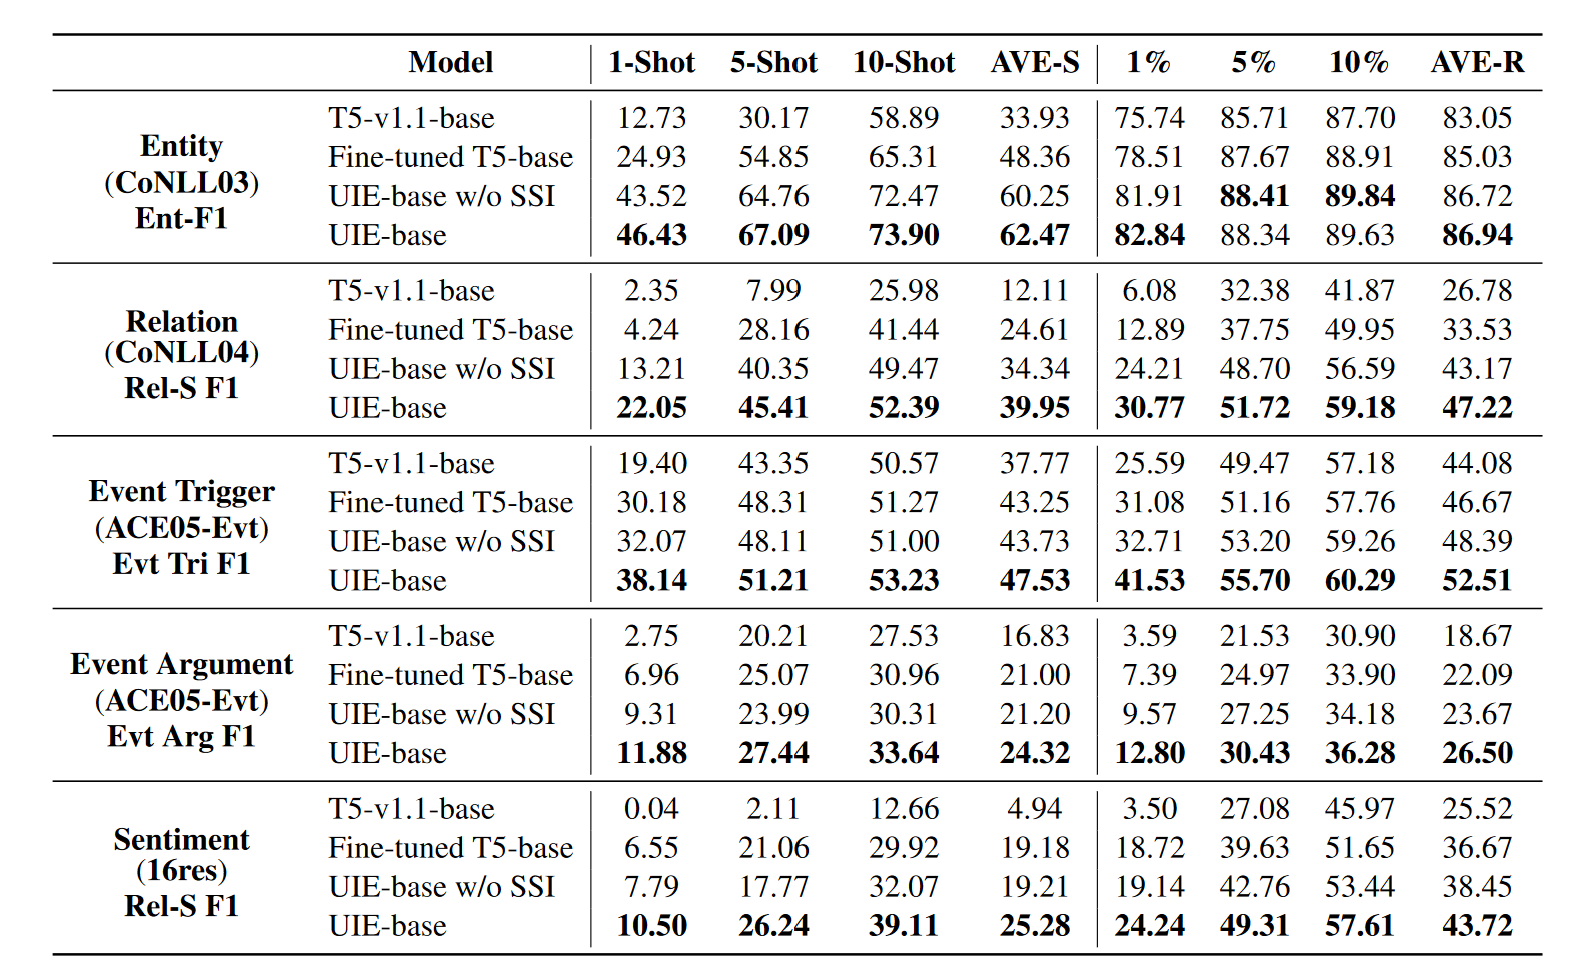
\includegraphics[width=1\linewidth]{UIE_results.png}
    \caption{(Lu et al., 2022)  Table 3}
    \label{UIE Results}
\end{figure}


\subsubsection{Instruct UIE}
UIE requires separate fine-tuning for different downstream tasks. This leads to the poor performance of UIE in low resources settings or facing new label schema which restricts application of UIE in real scenarios. The approach proposed by (Wang et al., 2023) aims to solve this by reformulating IE tasks as natural language generation problem by introducing a unified IE framework based on instruction tuning, which can uniformly model various information extraction tasks and capture the 	inter task dependency. The results demonstrated that InstructUIE achieves comparable performance to Bert in a supervised setting. The method outperformed current SoTA and GPT-3.5 in a zero shot scenario. 

The IE tasks are formulated as seq2seq tasks and every task instance is formatted with 4 properties. 
Instruction: Provides a guide on how to extract the relevant information from the input text and produce the desired output structure. 
Options: Are output labels constraints for a task they represent the set of possible outputs that can be generated by the model. For example: Relation types
Text: Input sentence of the task instance. 
The sequence is then fed into the pre-trained language model along with the task instructions and options, enabling the model to generate the desired output sequence for the task. 

\textbf{NER}
The model achieves an average F1 score of 85.19\% on 20 NER datasets, surpassing Bert’s 80.09\% where InstructUIE achieved 92.94\%. InstructUIE outperforms the Bert model on 17 of NER datasets. Among them the model outperforms Bert by more than 5 points on 8 datasets. The dataset with biggest gap is the broad twitter dataset where the different is of 25 points.
Relation Extraction
Model reaches an average of 67.98\% on the eight datasets of RE tasks, among which the NYT dataset reaches 90.47\% F1 score.
For the CoNLL2004 dataset, InstructUIE outperforms UIE by more than three points.

\textbf{Event extraction}
The model achieves SoTa on all datasets except for the event trigger F1 metric of the CASIE dataset. On the event trigger F1 metric, the InstructUIE reaches an average of 71.69 on these three dataset. On the event argument F1 metric, instructUIE beats three baseline models to reach SoTA on all three datasets. ACE2005 dataset reaches 72.94\%, 18 points higher than the UIE and 17 points higher than USM.

Overall, results demonstrate that InstructUIE achieves state-of-the-art results under supervised and zero settings and solves massive tasks using a single multi-task model.
\begin{figure}
    \centering
    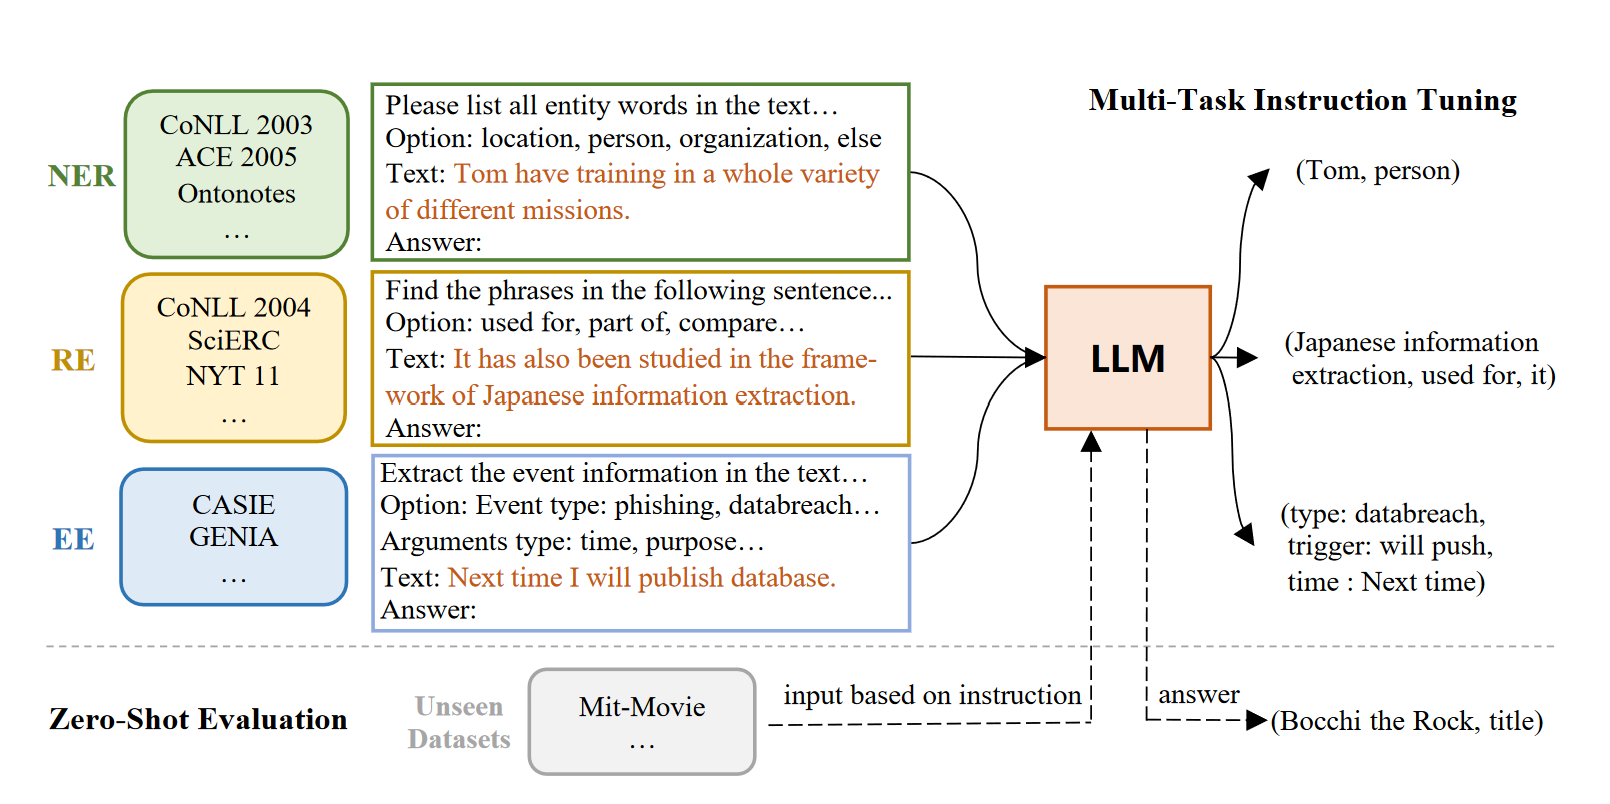
\includegraphics[width=1\linewidth]{InstructUIE.png}
    \caption{Wang et al. (2023) Figure 2}
    \label{Instruct UIE }
\end{figure}

\begin{figure}
    \centering
    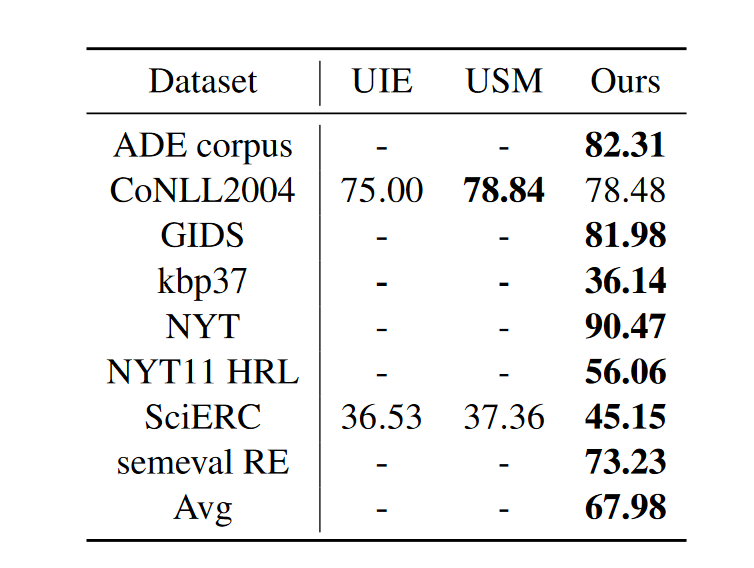
\includegraphics[width=0.75\linewidth]{InstructUIE_results.png}
    \caption{Wang et al. (2023)  Table 2}
    \label{Instruct UIE Results}
\end{figure}
\begin{figure}
    \centering
    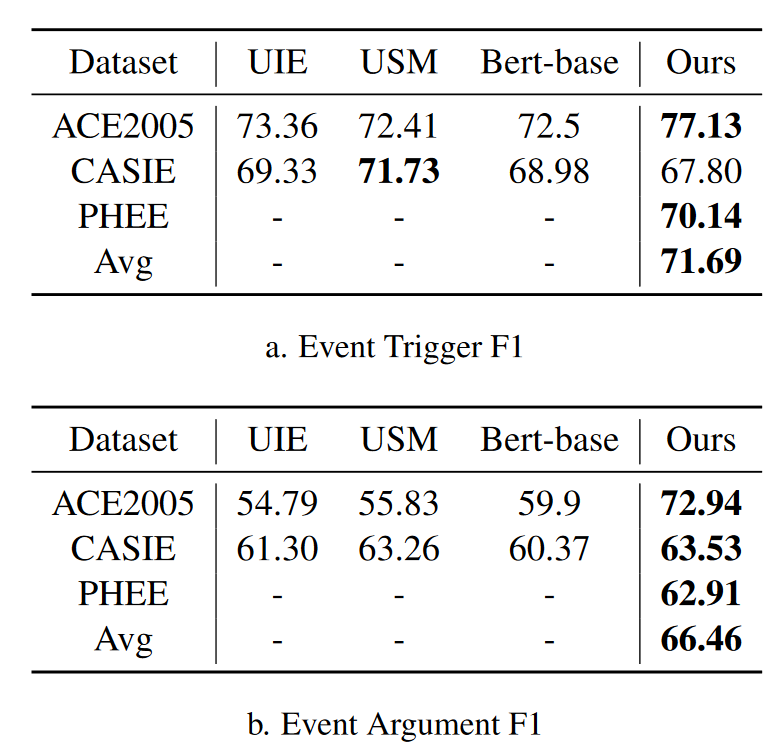
\includegraphics[width=0.5\linewidth]{InstructUIE_results2.png}
    \caption{Wang et al. (2023)  Table 3}
    \label{Instruct UIE Results 2}
\end{figure}
\subsection{Future research direction}
Future directions in relation extraction using large language models (LLMs) include several key areas of focus. Improved pre-training strategies, especially domain-specific techniques and the use of large-scale datasets, are crucial for enhancing performance. 

The evaluation of more complex datasets and the inclusion of multilingual datasets are essential for the advancement of RE. This could include developing models that can handle diverse and intricate linguistic structures across different languages, thereby enhancing the applicability of RE models in global contexts.

Despite significant progress at the sentence level, document-level RE remains a challenging area. Future research could explore more sophisticated approaches to aggregating evidence across entire documents, possibly incorporating techniques from other NLP tasks such as document summarization and coreference resolution.

Extending RE models to be more KB-aware (knowledge base-aware) can significantly improve their performance. Future work could focus on integrating external knowledge bases into RE models to enhance their ability to accurately extract and classify relations, especially in cases where the context or entities are not well-represented in the training data.

Building upon the concept of Universal Information Extraction (UIE), future research could aim to develop more comprehensive frameworks that unify various IE tasks, including entity linking, event extraction, and coreference resolution. This unification could facilitate better knowledge sharing between tasks and lead to more robust and versatile IE systems.

 
\section{Conclusion}
In this paper, we have surveyed recent advancements in Relation Extraction (RE), focusing on the impact of large language models (LLMs) and their role in transforming the field. The exploration of various techniques highlights the significant strides made through innovative approaches such as prompt design, alignment, and Universal Information Extraction (UIE). 

Our review emphasizes the pivotal role of LLMs in advancing RE tasks. Techniques like Chain of Thought (CoT) and Universal Information Extraction have demonstrated substantial improvements in performance by leveraging the sophisticated understanding and generation capabilities of these models. CoT, in particular, has shown that fine-tuning models with detailed, step-by-step reasoning can lead to impressive gains in accuracy. On the other hand, approaches like QA4RE and RAG4RE have showcased the potential of aligning RE with more prevalent tasks and integrating retrieval-based strategies to overcome limitations such as hallucination. 

The paper also identifies key challenges and future directions. Despite the progress, several areas remain ripe for exploration. For instance, the limited evaluation of more complex datasets and the need for improved methods to handle document-level RE highlight ongoing challenges. Additionally, the unification of various IE tasks through frameworks like UIE presents a promising direction for enhancing knowledge sharing and model efficiency.
Future research should focus on addressing these challenges by exploring alternative approaches to fine-tuning, expanding the applicability of frameworks like UIE to new contexts, and enhancing the robustness of models against issues like hallucination. Moreover, extending these methods to real-world, dynamic scenarios and incorporating multilingual datasets could further advance the field. 
In conclusion, the integration of LLMs into RE has opened new avenues for improving performance and efficiency. The continuous evolution of these models and techniques promises to drive further innovations, making RE more accurate and applicable across diverse domains. The ongoing efforts to refine these methods and address existing challenges will be crucial in advancing the state-of-the-art and achieving more comprehensive and reliable information extraction solutions.


\section{What did I learn from odyssey}
Doing odyssey for summer 2023 was my first step towards a career of research and a very hands-on experience of how research looks like. I was given weekly tasks which involved reading papers, identifying their key information and presenting it to my supervisor then discussing the next steps in the project. It was a very illuminating experience into the world of research. I would like to thank my supervisor Ms Yanfei Dong as she helped me navigate through the project, from deciding the project to helping me improve my presentation and writing skills by providing valuable feedback at every step and teaching me how to use research tools to my advantage and conduct a literature review.

\newpage

\bibliographystyle{vancouver}
\bibliography{sample}
\cite{*}



\end{document}